% 20181215
% Start this project
% 20181018
% "e:\MikTeX Portable\miktex\bin\pdflatex" butiran
% i:\texmfs\install\miktex\bin\pdflatex butiran
% Use in Chrome butiran.pdf#page=3&zoom=120,140,300
% Download again from https://miktex.org/download for
% portable edition -- not work while updating packages
% It requires proxy and solved through GUI and source of
% installer
% 20190129
% Create butiran-latex.bat for more convenient latexing.
% 20190507
% Start JS introduction for Kakakku
% 20190525
% Start MPSSS project at home
% 20190827 Start fi1101-40 for 2019-1 lecture.

% 20191017
% 1708 Restart butiran (textbook) project

\documentclass[10pt,a4paper,oneside]{book}

\usepackage{array}
\usepackage[dvipsnames]{xcolor}
\usepackage{listings}
\usepackage[hyphenbreaks]{breakurl}
%\usepackage[hyphens]{url}
\usepackage[breaklinks=true,colorlinks=true,urlcolor=blue]
	{hyperref}
\sloppy
\def\UrlBreaks{\do\/\do-}

\definecolor{codegreen}{rgb}{0,0.6,0}
\definecolor{codegray}{rgb}{0.5,0.5,0.5}
\definecolor{codepurple}{rgb}{0.58,0,0.82}
\definecolor{backcolour}{rgb}{0.98,0.98,0.96}

\definecolor{codeblue}{rgb}{0,0,0.8}

 
\lstdefinestyle{granularstyle}{
  backgroundcolor=\color{backcolour},   
  %commentstyle=\color{codegreen},
  keywordstyle=\color{magenta},
  numberstyle=\scriptsize\color{codegray},
  stringstyle=\color{codepurple},
  basicstyle=\small\ttfamily,
	identifierstyle  = \color{black},
  breakatwhitespace=false,         
  breaklines=true,                 
  captionpos=b,                    
  keepspaces=true,                 
  numbers=left,                    
  numbersep=5pt,                  
  showspaces=false,                
  showstringspaces=false,
  showtabs=false,                  
  tabsize=2,
  morekeywords = {var, for, function, return, if, else, using, namespace, case, switch, while, do, class, struct, break, friend},
  morekeywords = [2]{true, false}, % HERE : add remove the parenthesis
  keywordstyle = [2]\color{codeblue},
  morekeywords = [3]{html}, % HERE : add remove the parenthesis
  keywordstyle = [3]\color{codegreen},
  morekeywords = [4]{int, char, double, string, void, const, bool, long, enum},
  keywordstyle = [4]\color{magenta},
  morecomment = [l]{//},
  morecomment = [s]{/*}{*/},
  morecomment = [s]{/**}{*/},
	morecomment = [s]{<!-}{-->},
  commentstyle = \color{gray},
	moredelim = [l][\color{codegreen}]{\#}, % for #include in C++
  morestring = [b]',
  morestring = [b]",
  stringstyle = \color{purple},
	otherkeywords={
		<p>,</p>, <html>,</html>, <head>,</head>, <body>,</body>,
		<title>,</title>, <style>,</style>, <script>,</script>
	},
  keywordstyle = \color{codeblue},
}
\lstset{style=granularstyle}

\usepackage{tikz}

\renewcommand{\contentsname}{Isi}
\renewcommand{\chaptername}{}
\renewcommand{\tablename}{Tabel}
\renewcommand{\figurename}{Gambar}
\renewcommand{\lstlistingname}{Kode}

% 20181221
\usepackage{algorithm}
\usepackage{algpseudocode}
%\renewcommand{\thealgorithm}{Algoritma}
%\makeatletter\renewcommand{\ALG@name}{Algoritma}\makeatother
% 20181222
%\renewcommand\thealgorithm{\thechapter.\arabic{algorithm}} \@addtoreset{algorithm}{chapter} \makeatother
%\makeatletter\renewcommand{\ALG@name}{Algoritma \thechapter.} \@addtoreset{algorithm}{chapter}\makeatother
\renewcommand{\thealgorithm}{\arabic{chapter}.\arabic{algorithm}}

% 201812122
\usepackage[latin1]{inputenc}
\usepackage{tikz}
\usetikzlibrary{shapes,arrows}
\usetikzlibrary{positioning}
% 20181223
\usetikzlibrary{plotmarks}
\usepackage{pgfplots}
%\usepackage{pgfplotstable}
\usepackage{pgfplotstable,filecontents} % 20190108

% url http://www.texample.net/tikz/examples/simple-flow-chart/ [20181222]
% Define block styles
\tikzstyle{decision} = [diamond, draw, fill=yellow!20, text width=3.5em, text badly centered, inner sep=0pt]
\tikzstyle{block} = [rectangle, draw, fill=blue!20, text width=5em, text centered, rounded corners, minimum height=2em]
\tikzstyle{line} = [draw, -latex']
\tikzstyle{cloud} = [draw, ellipse, minimum height=2em]

\tikzstyle{point} = [draw, circle, minimum size=5pt, inner sep=0pt, outer sep=0pt]

% 20181229
\usepackage{multirow}

% 20181224
\usepackage{amssymb}

% 20181215 -- not work
\makeatletter

\def\@listi{%
	% default setting for base LaTeX classes at 10 pt:
	\parsep 4pt plus 2pt minus 1pt
	\topsep 8pt plus 2pt minus 4pt
	\itemsep 4pt plus 2pt minus 1pt
	% your setting
	\parskip 1em plus 1pt minus 1pt
}

\makeatother
% -----

\usepackage{verbatim}

% 20190106 --> \substack{ \\ }
\usepackage{amsmath}
\renewcommand{\algorithmicrequire}{\textbf{Input:}}
\renewcommand{\algorithmicensure}{\textbf{Output:}}

\setlength{\parindent}{0pt}
\setlength{\parskip}{0.5em}

% 20190109
\DeclareMathOperator{\atan}{atan}

% 20190130
% https://tex.stackexchange.com/a/222411
\usepackage{enumerate}
% https://tex.stackexchange.com/a/33798
\algnewcommand{\algorithmicgoto}{\textbf{go to}}%
\algnewcommand{\Goto}[1]{\algorithmicgoto~\ref{#1}}%

% 20190203 -- https://tex.stackexchange.com/a/118217
%\usepackage{mathtools}
%\DeclarePairedDelimiter\ceil{\lceil}{\rceil}
%\DeclarePairedDelimiter\floor{\lfloor}{\rfloor}
% cancel it's not scaled

% 20190217 -- https://tex.stackexchange.com/a/400752/180784
\setlength{\fboxsep}{2pt}

\title{butiran \\ \ \\ {\normalsize \url{https://osf.io/kzs4f/} } }
\author{Sparisoma Viridi}
\date{2019}

% 20190721 -- https://tex.stackexchange.com/a/417698/180784
\def\tmp#1 #2\relax{#1}
\setbox0=\hbox{$\xdef\intfont{%
    \expandafter\tmp\fontname\textfont3\expandafter\space\space\relax}$}
\font\tmp=\intfont\space at10pt\relax
\setbox0=\hbox{$\textfont3=\tmp \displaystyle \int$}
\dimen0=\ht0 \advance\dimen0 by\dp0 \divide\dimen0 by10 
\xdef\intsize{\the\dimen0}

\def\dividedimen (#1/#2){\expandafter\ignorept\the
   \dimexpr\numexpr\number\dimexpr#1\relax
   *65536/\number\dimexpr#2\relax\relax sp\relax
}
{\lccode`\?=`\p \lccode`\!=`\t  \lowercase{\gdef\ignorept#1?!{#1}}}

\def\flexibleint{\def\fxintL{}\def\fxintU{}\futurelet\next\fxintA}
\def\fxintA{\ifx\next_\expandafter\fxintB\else\expandafter\fxintC\fi}
\def\fxintB_#1{\def\fxintL{#1}\fxintC}
\def\fxintC{\futurelet\next\fxintD}
\def\fxintD{\ifx\next^\expandafter\fxintE\else\expandafter\fxintF\fi}
\def\fxintE^#1{\def\fxintU{#1}\fxintF}
\def\fxintF#1{\begingroup
   \setbox0=\hbox{$\displaystyle{#1}$}%
   \dimen0=\ht0 \advance\dimen0 by\dp0
   \setbox1=\hbox{$\vcenter{\copy0}$}%
   \font\tmp=\intfont\space at\dividedimen(\dimen0/\intsize)pt
   \lower\dimexpr\dp0-\dp1\hbox{%
      $\textfont3=\tmp \displaystyle\int_{\fxintL}^{\fxintU}$}
   \box0
   \endgroup
}


\begin{document}

%\maketitle % 20191017 beg, end

\tableofcontents

\frontmatter

\mainmatter

%% 20190826
% It will be increased by 1 after \chapter
\setcounter{chapter}{0}
% Set this page number
\setcounter{page}{1}


\chapter{Pendahuluan}
Secara umum banyak sistem fisis yang dapat dimodelkan dengan menggunakan agen baik berupa butiran-butiran atau entitas lain yang saling berinteraksi baik secara permanen (rentang jauh) ataupun hanya sesekali (rentang dekat). Tulisan ini akan membahas hal tersebut yang dilengkapi dengan contoh implementasinya menggunakan pustaka \verb|abm-x|\footnote{url \url{https://github.com/dudung/abm-x} [20200605]} yang ditulis dalam bahasa pemrograman JavaScript (JS) dan lainnya.


%
\section{Berkas-berkas utama}
Terdapat beberapa berkas yang diperlukan untuk menjalankan pustaka \verb|abm-x|, yaitu berkas HTML dan JS yang dalam contoh ini bernama \verb|hello.html| dan \verb|hello.js|, serta versi terkompresi dari pustaka sebelumnya dengan nama berkas \verb|butiran.min.js| yang dapat diperoleh dari folder \verb|dist|.

\lstinputlisting[label={lst:hello.html}, caption={Berkas {\tt hello.html}.}, linerange={1}, firstnumber=1]{01/hello.html}

Kode \ref{lst:hello.html} memerlukan dua berkas yaitu versi terkompresi dari pustaka \verb|butiran.js| dan berkas \verb|hello.js|.

\lstinputlisting[label={lst:hello.js}, caption={Berkas {\tt hello.js}.}, linerange={1}, firstnumber=1]{01/hello.js}

Isi dari berkas \verb|hello.js| diberikan dalam Kode \ref{lst:hello.js}. Beris 18 akan menuliskan frasa "Hello world!" pada konsol perambat internet, e.g. Google Chrome, baris 19 mendefinisikan suatu besaran berjenis \verb|Vect3| dan baris 20 menuliskan isinya. Kelas \verb|Vect3| merupakan bagian dari pustaka \verb|butiran.js| yang bila tidak ada pesan kesalahan menunjukkan bahwa pustaka ini telah sukses disertakan.

\begin{figure}[H]
\centering
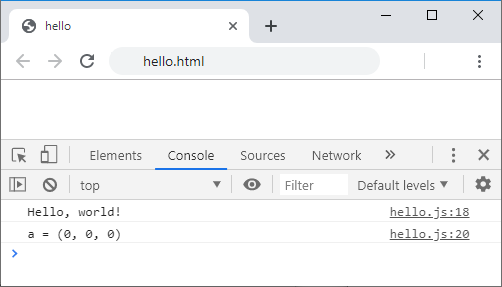
\includegraphics[width=10cm]{01/hello.png}
\caption{\label{fig:hello} Tampilan berkas {\tt hello.html} dalam peramban internet Google Chrome.}
\end{figure}

Untuk melihat konsol pada Google Chrome digunakan kombinasi tombol CTRL + SHIFT + J, yang berbeda-beda untuk setiap peramban internet.\footnote{"How to open the developer console", Airtable, url \url{https://support.airtable.com/hc/en-us/articles/232313848-How-to-open-the-developer-console} [20191017].} Dalam Gambar \ref{fig:hello} pada bagian kanan tercantum baris keberapa pada berkas \verb|hello.js| yang menghasilkan keluaran tersebut. Dengan menggunakan informasi ini pengguna dapat melacak hasil keluaran yang diperoleh.

Untuk berikutnya terkait dengan konsol bila tidak benar-benar diperlukan tampilan dalam peramban internet tidak akan ditayangkan, melainkan cukup hanya bagian teksnya tersebut

\begin{lstlisting}[numbers=none]
Hello, world!                                  hello.js:18
a = (0, 0, 0)                                  hello.js:20
\end{lstlisting}

yang ditampilkan.


%
\section{Catatan}
Rujukan, terutama yang yang bersumber dari internet, akan disertakan sebagai catatan kaki.    % 20191017 beg
%\include{02/vector}   % 20191017 beg
%\include{03/projects} % 20191211 beg

\appendix

\backmatter

\end{document}

% References
% 5. LaTeX arrows -- 20190224
% url http://www.sascha-frank.com/Arrow/latex-arrows.html

% 1. tikzpicture file columns -- 20190217
% url https://tex.stackexchange.com/a/30383/180784
% 2. plot every nth point only -- 20190217
% url https://tex.stackexchange.com/a/47800/180784
% 3. Line type -- 20190217
% url https://tex.stackexchange.com/a/327983/180784
% 4. Legend position -- 20190217
% url https://tex.stackexchange.com/a/295571/180784


